\frontmatter

\title{\caps{Intensional
    Semantics}\\[36pt]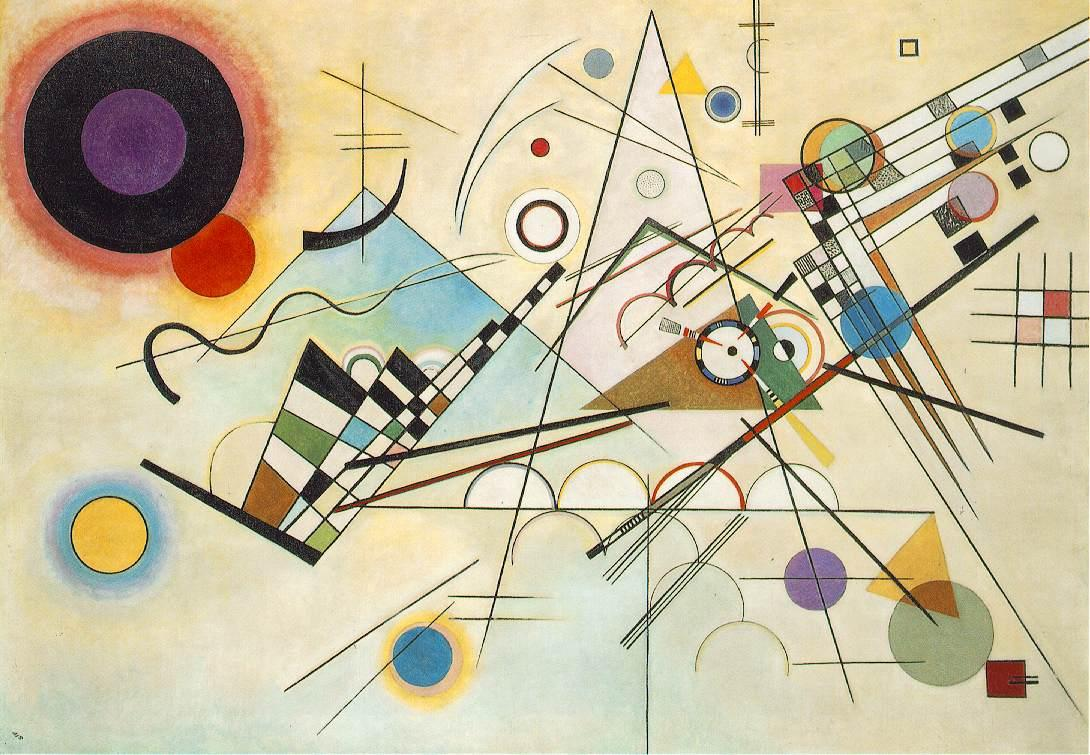
\includegraphics[width=\textwidth]{kandinsky-1923-composition-viii.jpg}}
\author{\caps{Kai von Fintel}\and{\caps{Irene Heim}}}
\date{\caps{1997 -- $\infty$}\\[18pt] [last changed on \today]}

\pagestyle{empty}


\maketitle

\cleardoublepage

\section*{About these lecture notes}

\plainbreak{1} 

These lecture notes have been evolving for years now, starting with some old
notes from the early 1990s by Angelika Kratzer, Irene Heim, and Kai von Fintel,
which have since been modified and expanded many times by Irene and/or Kai.

\plainbreak{1} 

We encourage the use of these notes in courses at other institutions. Of course,
you need to give full credit to the authors and you may not use the notes for
any commercial purposes. If you use the notes, we would like to be notified and
we would very much appreciate any comments, criticism, and advice on these
materials.

\plainbreak{1}

Cite as follows\\[6pt]\null\hfill
von Fintel, Kai \amp\ Irene Heim. 1997--2017. Intensional Semantics. MIT.

\medskip

\noindent Link to the latest full version (not necessarily up-to-date):\\[6pt]
                                             \null\hfill\url{http://kvf.me/intensional}
\medskip
                                            
\noindent GitHub repository with the current \&\ up-to-date development version:\\[6pt]
            \null\hfill\url{https://github.com/fintelkai/fintel-heim-intensional-notes}

\medskip

\noindent Most recent homepage of the class these notes are designed for:\\[6pt]
\null\hfill\url{http://kvf.me/advsem}

\medskip

\noindent Cover image: \url{https://www.guggenheim.org/artwork/1924}.

\vfill

\noindent Kai von Fintel \amp\ Irene Heim\\
Department of Linguistics \amp\ Philosophy\\
Massachusetts Institute of Technology\\
77 Massachusetts Avenue\\
Cambridge, \textsc{ma} 02139-4307\\
\textsc{United States of America} 

\plainbreak{1}

\href{mailto:fintel@mit.edu}{fintel@mit.edu}, \href{mailto:heim@mit.edu}{heim@mit.edu}

\cleardoublepage

\null
\vfill \ba 

\section*{Acknowledgments}

Thanks to generations of students in our classes. Thanks to colleagues who have
used these notes in their classes. Here's an almost certainly incomplete list of
people who have helped us in some way or other with these notes (telling us
about typos, asking questions, pointing out issues, etc.): Paul Elbourne, Nick
Fleisher, Graeme Forbes, Adam Goodkind, Aaron Jacobs, Magda Kaufmann, Ezra
Keshet, Angelika Kratzer, Manfred Kupffer, Eric Mack, Yuliya Manyakina, Liz
Smeets, Vesela Tihomirova Simeonova, Ede Zimmermann.

\section*{Some advice}
\begin{enumerate}
\item These notes presuppose familiarity with the material, concepts, and
  notation of the Heim \amp\ Kratzer textbook.
\item There are numerous exercises throughout the notes. It is highly
  recommended to do all of them and it is certainly necessary to do so if you at
  all anticipate doing semantics-related work in the future.
\item The notes are designed to go along with explanatory lectures. You should
  ask questions and make comments as you work through the notes.
\item Students with semantic ambitions should also at an early point start
  reading supplementary material (as for example listed at the end of each
  chapter of these notes).
\item Prospective semanticists may start thinking about how \emph{they} would
  teach this material.
\item For more advice along these lines, see
  \url{http://kaivonfintel.org/prerequisites/}.
\end{enumerate}

\ab 
\vfill\null

\newpage\hbox{}
\vfill{\scshape\caps{--- This page intentionally left blank ---}}
\vfill\hbox{}\thispagestyle{cleared}

\cleardoublepage

\tableofcontents*

\cleardoublepage